% \documentclass[a4paper,journal]{IEEEtran}
\documentclass[conference]{IEEEtran}
%% INFOCOM 2013 addition:
\makeatletter
\def\ps@headings{%
\def\@oddhead{\mbox{}\scriptsize\rightmark \hfil \thepage}%
\def\@evenhead{\scriptsize\thepage \hfil \leftmark\mbox{}}%
\def\@oddfoot{}%
\def\@evenfoot{}}
\makeatother
\pagestyle{headings}
\usepackage{psfrag}

% \usepackage{auto-pst-pdf}

\usepackage[utf8]{inputenc}
\usepackage{graphicx}
\usepackage{float}
\usepackage{color, colortbl}
\usepackage{xcolor}
\usepackage{array}
\usepackage{multirow}
\usepackage{footnote}
\usepackage{cite}
%The below is used to add notes to tables without disrupting the IEEEtran format
\usepackage{threeparttable}

% Disable below if wanting to comply exclusively to conference mode of IEEEtran
% \IEEEoverridecommandlockouts

\makesavenoteenv{tabular}

%Ignores \vbox errors below the level of 10000
% \vbadness=10000



\begin{document}
%opening
 \title{Fairness in Collision-free WLANs}


%A more simple output, useful when involving people from different affiliations
  \author{
      \IEEEauthorblockN{Luis Sanabria-Russo\IEEEauthorrefmark{0}, Jaume Barcelo\IEEEauthorrefmark{0}, Boris Bellalta\IEEEauthorrefmark{0}}\\
      \IEEEauthorblockA{\IEEEauthorrefmark{0}Universitat Pompeu Fabra, Barcelona, Spain
      \\\{luis.sanabria, jaume.barcelo, boris.bellalta\}@upf.edu}
  }

%This is the style of three columns, as indicated in IEEEtran
% \author{\IEEEauthorblockN{Luis Sanabria-Russo}
%  \IEEEauthorblockA{Department of Information\\
%  and Communications Technologies\\
%  Universitat Pompeu Fabra\\
%  Barcelona, Spain\\
%  Email: luis.sanabria@upf.edu}
%  \and
%  \IEEEauthorblockN{Jaume Barcelo}
%  \IEEEauthorblockA{Department of Information\\
%  and Communications Technologies\\
%  Universitat Pompeu Fabra\\
%  Barcelona, Spain\\
%  Email: cristina.cano@upf.edu}
%  \and
%  \IEEEauthorblockN{Boris Bellalta}
%  \IEEEauthorblockA{Department of Information\\
%  and Communications Technologies\\
%  Universitat Pompeu Fabra\\
%  Barcelona, Spain\\
%  Email: boris.bellalta@upf.edu}}


\maketitle

\begin{abstract}

\boldmath It is possible to achieve a collision-free state implementing Carrier Sense Multiple Access with Enhanced Collision Avoidance (CSMA/ECA). It differs from CSMA/CA in choosing a deterministic (instead of random) backoff after successful transmissions. Also in CSMA/ECA, contenders keep the increased length of the contention window even after a successful transmission, what results in an uneven distribution of the channel access time. This fairness issue is assessed in this work by adjusting the number of packets each contender is allowed to transmit on each opportunity. Results show a totally distributed, collision-free and fair protocol capable of achieving higher levels of throughput than those of the conventional CSMA/CA.

%On this work, this fairness issue is assessed and it is revealed how by adjusting the number of packets transmitted on each opportunity. Results show a totally distributed, collision-free and fair protocol capable of achieving higher levels of throughput than those of the conventional CSMA/CA.

%Furthermore, the enhanced CSMA/E2CA has stickiness degrees, which refer to number deterministic backoffs used after each successful transmission and account for shorter convergence time towards a collision-free state. Implementing CSMA/E2CA in a totally distributed way revealed the unfair nature of the protocol. This abstract introduces the concept of Fair Share as a way to leverage this issue, which consist of adapting the number of packets to be transmitted accordingly with the backoff stage of each node. Results show a totally distributed, collision-free and fair protocol capable of achieving higher levels of throughput than those of the conventional CSMA/CA.

\end{abstract}

\begin{IEEEkeywords}
Wireless, MAC, Collision-free, CSMA/ECA.
\end{IEEEkeywords}

\section{Introduction} \label{introduction}
  Carrier Sense Multiple Access with Enhanced Collision Avoidance (CSMA/ECA)~\cite{CSMA_ECA} achieves less collisions and outperforms CSMA/CA in most typical scenarios. This is done by picking a deterministic backoff after each successful transmission. CSMA/E2CA introduces stickiness in the process by setting the number of times a deterministic backoff is used after each successful transmission, which accounts for a reduced convergence time towards a collision free state.

Stickiness can reduce the convergence time by orders of magnitude when the number of contenders $\eta$ is less or equal than the expectation of the random backoff used in CSMA/CA, $C$. The same constraint is valid for improvements in throughput, as can be appreciated in Figure~\ref{fig:throughput}.

\begin{figure}[htbp]
  \centering
  \includegraphics[width=0.7\linewidth, angle = -90]{figures/throughput/throughput.eps}
  \caption{Throughput and how it is affected when $\eta \geq C$
  \label{fig:throughput}}
\end{figure}

In Figure~\ref{fig:throughput}, when $\eta \geq C$ the system is overcrowded with contenders and the collision-free state is compromised. As more contenders are introduced, 

\section{A descentralized and fair CSMA/ECA} \label{csmae2ca}
  There are numerous reasons why CSMA/ECA is more useful when modeled as a decentralized protocol. One being the removal of the Access Point (AP) as a single point of failure. Also, AP Beacons are no longer used as a control measure to estimate the number of contenders in the network, which in turn reduces the overall convergence time.

% In order to model the protocol, it is treated a Decentralized Constraint Satisfaction (DCS) problem~\cite{DCSP, DCSP-E2CA} using the ACK as the only feedback information that identifies a successful transmission.

In an overcrowded CSMA/ECA ($\eta>C$), colliding nodes will double $CW$ each time and reset it ($CW=CW_{min}$) upon each transmission success, augmenting its collision probability. This behavior accounts for the throughput reduction in Figure~\ref{fig:throughput}.

In order to leverage this issue, CSMA/ECA forces nodes to \emph{stick} to its backoff stage (or \emph{stage stickiness} from here on), $m$. That is, $CW$ is no longer reset after a successful transmission; resulting in a greater system capacity because of the larger $CW$. This leads to a collision-free state while $\eta\leq C_{m}$, where $C_{m}$ accounts for $C$ in Eq.~\ref{eq:capacity} computed with a $CW$ in a backoff stage $m$.

Having a greater system capacity ($C_{m} > C$) accounts for more nodes being able to achieve a collision-free state. Nevertheless, in a $\eta\leq C_{m}$ scenario, contenders may have different deterministic backoff counters ($bo_{d}$) which provoke some nodes to access the channel more often than others. This fairness issue is averted with \emph{fair share}.

This mechanism consist on allowing each contender to send $2^{m}$ packets every time its backoff expires ($bo_{d}=0$), making sure that contenders with longer backoff are compensated proportionally.

Figure~\ref{fig:fairShare}, depicts how CSMA/ECA with stage stickiness and fair share achieves greater throughput than CSMA/CA, maintaining a collision-free state and being fair (Jain's Fairness Index~\cite{JFI}~(JFI) equals 1).

%If $\eta > C$ and under saturation (all contenders have something to transmit, all the time), $\eta - C$ contenders are forced to choose a random backoff, given that there are no unpicked slots available for transmission. This in turn provokes collisions on the $C$ remaining nodes that picked a slot using a deterministic backoff~\cite{CSMA_ECA}. 

%CSMA/E2CA manages this issue forcing the nodes to \emph{stick} to a deterministic backoff. That is, the contenders will choose a deterministic backoff two times after a successful transmission. If two consecutive collisions occur, then the contender will be forced to double its contention window (by incrementing the backoff stage, $m$ in Eq.~\ref{eq:backoff_stage}) and to pick a random backoff. This results in a faster convergence to a collision-free state, but at the same time reduces the fairness of the protocol given that some contenders may have to wait more than others to access the channel.

%\begin{equation} \label{eq:backoff_stage}
%	W = 2^{m}CW_{min},\ m\in[0,...,5]
%\end{equation}

%\subsection{Ensuring fairness}
%Under CSMA/E2CA, nodes may have different contention windows ($W$ in Eq.~\ref{eq:backoff_stage}), this means that some arbitrary contenders have to wait more than others in order to access the channel; compromising the fairness of the protocol. To leverage this issue, nodes are set to transmit $2^{m}$ packets every time their backoff counter expires. That is, if a contender doubled its contention window, then it will also double the packets that are going to be transmitted on the next opportunity. This fairness mechanism for CSMA/E2CA is called Fair Share from here on.

\begin{figure}[htbp]
  \centering
  \includegraphics[width=0.7\linewidth, angle = -90]{figures/throughput/CSMA-E2CA_w_fairShare.eps}
  \caption{Throughput and Jain's Fairness Index when implementing Fair Share in CSMA/E2CA
  \label{fig:fairShare}}
\end{figure}

%In Figure~\ref{fig:fairShare} it is appreciated through the estimation of the Jain's Fairness Index~\cite{JFI} that by implementing Fair Share every contender receives almost the same service time, therefore the system is considered fair.

\section{Future directions} \label{future}
  Our future work will be focused on implementing CSMA/ECA in cheap commodity hardware. Doing so will open the door for evaluation under more realistic scenarios as well as provide insight on different communication aspects, for example those regarding channel errors, delay, synchronization and coexistence with other access protocols. Nevertheless, this is not a trivial task given that in requires flexible network interface hardware which is not commonly provided by manufacturers. 

Project FLAVIA~\cite{FLAVIA}
  
\bibliographystyle{Classes/IEEEtran}
\bibliography{IEEEabrv,ref}
  
\end{document}